
%%%%%%%%%%%%%%%%%%%%%%%%%%%%%%%%%%%%%%%%%%%%%%%%%%%%%%%%%%%%%%%%%%%%%%%%%%%%%%%%%%%%%%%
%%%%%%%%%%%%%%%%%%%%%%%%%%%%%%%%%%%%%%%%%%%%%%%%%%%%%%%%%%%%%%%%%%%%%%%%%%%%%%%%%%%%%%%
% 
% This top part of the document is called the 'preamble'.  Modify it with caution!
%
% The real document starts below where it says 'The main document starts here'.

\documentclass[12pt]{article}

\usepackage{amssymb,amsmath,amsthm}
\usepackage[top=1in, bottom=1in, left=1.25in, right=1.25in]{geometry}
\usepackage{fancyhdr}
\usepackage{enumerate}
\usepackage{listings}
\usepackage{graphicx}
\usepackage{float}

\usepackage{mwe}
\usepackage{caption}
\usepackage{subcaption}
% Comment the following line to use TeX's default font of Computer Modern.
\usepackage{times,txfonts}



\makeatletter
\renewcommand*\env@matrix[1][*\c@MaxMatrixCols c]{%
  \hskip -\arraycolsep
  \let\@ifnextchar\new@ifnextchar
  \array{#1}}
\makeatother

\newtheoremstyle{homework}% name of the style to be used
  {18pt}% measure of space to leave above the theorem. E.g.: 3pt
  {12pt}% measure of space to leave below the theorem. E.g.: 3pt
  {}% name of font to use in the body of the theorem
  {}% measure of space to indent
  {\bfseries}% name of head font
  {:}% punctuation between head and body
  {2ex}% space after theorem head; " " = normal interword space
  {}% Manually specify head
\theoremstyle{homework} 

% Set up an Exercise environment and a Solution label.
\newtheorem*{exercisecore}{Exercise \@currentlabel}
\newenvironment{exercise}[1]
{\def\@currentlabel{#1}\exercisecore}
{\endexercisecore}

\newcommand{\localhead}[1]{\par\smallskip\noindent\textbf{#1}\nobreak\\}%
\newcommand\solution{\localhead{Solution:}}

%%%%%%%%%%%%%%%%%%%%%%%%%%%%%%%%%%%%%%%%%%%%%%%%%%%%%%%%%%%%%%%%%%%%%%%%
%
% Stuff for getting the name/document date/title across the header
\makeatletter
\RequirePackage{fancyhdr}
\pagestyle{fancy}
\fancyfoot[C]{\ifnum \value{page} > 1\relax\thepage\fi}
\fancyhead[L]{\ifx\@doclabel\@empty\else\@doclabel\fi}
\fancyhead[C]{\ifx\@docdate\@empty\else\@docdate\fi}
\fancyhead[R]{\ifx\@docauthor\@empty\else\@docauthor\fi}
\headheight 15pt

\def\doclabel#1{\gdef\@doclabel{#1}}
\doclabel{Use {\tt\textbackslash doclabel\{MY LABEL\}}.}
\def\docdate#1{\gdef\@docdate{#1}}
\docdate{Use {\tt\textbackslash docdate\{MY DATE\}}.}
\def\docauthor#1{\gdef\@docauthor{#1}}
\docauthor{Use {\tt\textbackslash docauthor\{MY NAME\}}.}
\makeatother

% Shortcuts for blackboard bold number sets (reals, integers, etc.)
\newcommand{\Reals}{\ensuremath{\mathbb R}}
\newcommand{\Nats}{\ensuremath{\mathbb N}}
\newcommand{\Ints}{\ensuremath{\mathbb Z}}
\newcommand{\Rats}{\ensuremath{\mathbb Q}}
\newcommand{\Cplx}{\ensuremath{\mathbb C}}
%% Some equivalents that some people may prefer.
\let\RR\Reals
\let\NN\Nats
\let\II\Ints
\let\CC\Cplx
%%%%%%%%%%%%%%%%%%%%%%%%%%%%%%%%%%%%%%%%%%%%%%%%%%%%%%%%%%%%%%%%%%%%%%%%%%%%%%%%%%%%%%%
%%%%%%%%%%%%%%%%%%%%%%%%%%%%%%%%%%%%%%%%%%%%%%%%%%%%%%%%%%%%%%%%%%%%%%%%%%%%%%%%%%%%%%%
% 
% The main document start here.

% The following commands set up the material that appears in the header.



%  \textbf{Code:}
%  \begin{center}
%  \lstinputlisting[basicstyle = \footnotesize]{}
%  \end{center}
%  
%  \begin{footnotesize}
%  \begin{verbatim}
%    
%  \end{verbatim}
%  \end{footnotesize}
%  
%  
%  \begin{figure}[H]
%    \begin{center}
%      \caption{}
%    \includegraphics[width = \textwidth]{}
%    \end{center}
%  \end{figure}




\doclabel{Stat 461: Homework 9}
\docauthor{Stefano Fochesatto}
\docdate{\today}

\begin{document}
\begin{exercise}{1} First input the data from Appendix One. All explanatory 
variables $x_1 \dots x_8$ are continuous. The response is spec which has values form 0 to 1. 

\begin{enumerate}
  \item[a.] Perform a logistic regression with all the variables. Does it fit significantly better than the null model? Us AIC values and also use 
  deviances. [The likelihood ratio test comparing two nested models (one has additional variables) is performed by
  taking the difference of the deviances and getting a p-value with the command: pchisq(devianceDifference, df, lower.tail=FALSE), where df
  is the number of additional explanatory variables in the more complicated model.]\\
  \solution Fitting both models, we get the following AIC and deviances. 
  \begin{center}
  \begin{tabular}{|c||c|c| }
    \hline
    Model & Deviance &  AIC \\
    \hline 
    \hline
    Full Model& 16.059 & 34.059 \\
    Null Model& 55.352 & 57.352 \\
    \hline
   \end{tabular}
  \end{center}
  Performing a likelihood ratio test we achieved a p-value of 4.3377e-06, at an $\alpha = .05$ significance level we reject the null hypothesis and conclude that 
  the full model is a significant improvement over the null model. 

      \textbf{Code:}
      \begin{center}
      \lstinputlisting[basicstyle = \footnotesize]{r1.txt}
      \end{center}
  \vspace{.15in}





  \item[b/c.] Now try to toss out variables one at a time until you get an optimal model. Make sure you tell me how you decided which variables to
  remove.\\
  \solution Throughout the Regression and Anova we used stepwise regression (Forward selection or Backward elimination) using AIC as our fitting criteria. We also explored regularization methods like LASSO. 
  Instead of removing each variable one at a time, we can use the bestGLM package to automatically consider every combination of variables (the docs call this method complete enumeration) 
  and pick from a variety of fitting criteria, such as AIC, BIC, and Cross-Validation. Checking for all three fitting criteria we find that the model including only $x1$ and $x8$ as predictors is the best.\\ 
  
  \textbf{Code:}
  \begin{center}
  \lstinputlisting[basicstyle = \footnotesize]{r2.txt}
  \end{center}
  \vspace{.15in}



  \item[d.] Next, make a table of actual spec vs predicted spec. Use the code 'table(spec, predict(spec)>0)'. How well does the model do at separating
  the two groups? From the table in (c), compute the sensitivity and specificity. Why did I pick predict(spec) >0 (hint: this isn't the probability).\\
  \solution When constructing a logistic regression, one must select a threshold which converts the output of the regression into class labels. This can 
  be influenced by priors and or costs of misclassification. Generally we want to construct a classifier which maximizes the area under the ROC curve or AUC and we choose the threshold
  by picking a point along the ROC curve (there are several methods for do this, picking the point with the smallest distance from (0,1) works 
  for minimizing misclassification where costs are the same). Constructing the confusion matrix for our best fitting model we get the following table, 
  \begin{center}
    \begin{tabular}{|c||c|c| }
      \hline
       & 0 &  1 \\
      \hline 
      \hline
      0& 16 & 2 \\
      1& 3 & 19 \\
      \hline
     \end{tabular}
    \end{center}
    Sensitivity is computed with the following, 
    \begin{equation*}
      \text{Sensitivity} = \dfrac{\text{True Positive}}{\text{True Positive + False Negative}} = \dfrac{16}{16 + 3} = .842.
    \end{equation*}
    Specificity is computed with the following, 
    \begin{equation*}
      \text{Specificity} = \dfrac{\text{True Negative}}{\text{True Negative + False Positive}} = \dfrac{19}{19 + 2} = .905.
    \end{equation*}
    \textbf{Code:}
    \begin{center}
    \lstinputlisting[basicstyle = \footnotesize]{r3.txt}
    \end{center}
 

  \end{enumerate}
\end{exercise}
\vspace{1in}


\begin{exercise}{2}  In this problem you'll "hand-make" an ROC curve. For the data in Problem One, repeat the table command for a variety of cutoff values (not just
  0). Use a cutoff of -3, -2, -1, 0, 1, 2, 3. Now compute the specificity and selectivity* for each table. Finally, plot an ROC curve. What is this curve
  used for?\\
  \solution Generating the ROC curve with the following code we find that an optimal value to threshold, with no prior information about misclassification costs is -.01. 
  The following code generates the confusion matrix for threshold in the range of -4 to 4, and computes the specificity and sensitivity. We decided to use the threshold which is 
  closest to (0,1) on the ROC curve. The ROC curve is used to evaluate threshold values, and also compare performance between models (using AUC).
  \begin{figure}[H]
    \begin{center}
      \caption{ROC Curve for the Best Logistic Regression Model}
    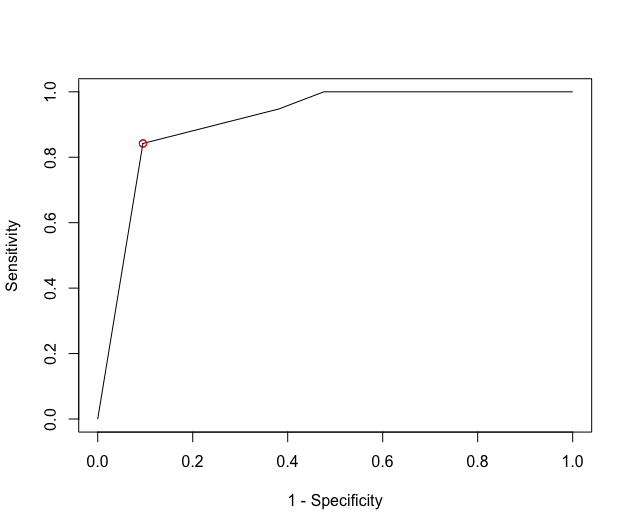
\includegraphics[width = \textwidth]{Rplot.png}
    \end{center}
  \end{figure}
  \textbf{Code:}
  \begin{center}
  \lstinputlisting[basicstyle = \footnotesize]{r4.txt}
  \end{center}n
\end{exercise}
\vspace{1in}



\begin{exercise}{3} Get the dataset from the top of the handout 'March 23 Lin. Disc. and Logistic Reg.'. Use multinomial (aka multivariate) logistic regression to
  classify the three groups. Use a test/train approach to validate the resulting classification.\\
  \solution Using the multinom() function from the nnet package we can fit a multinomial logistic regression to the data from the March Handout. Recall that the data overlapped 
  a lot, and an lda analysis only managed to attain an accuracy of 79.08\%. 
  \begin{figure}[H]
    \begin{center}
      \caption{Data From March Handout}
    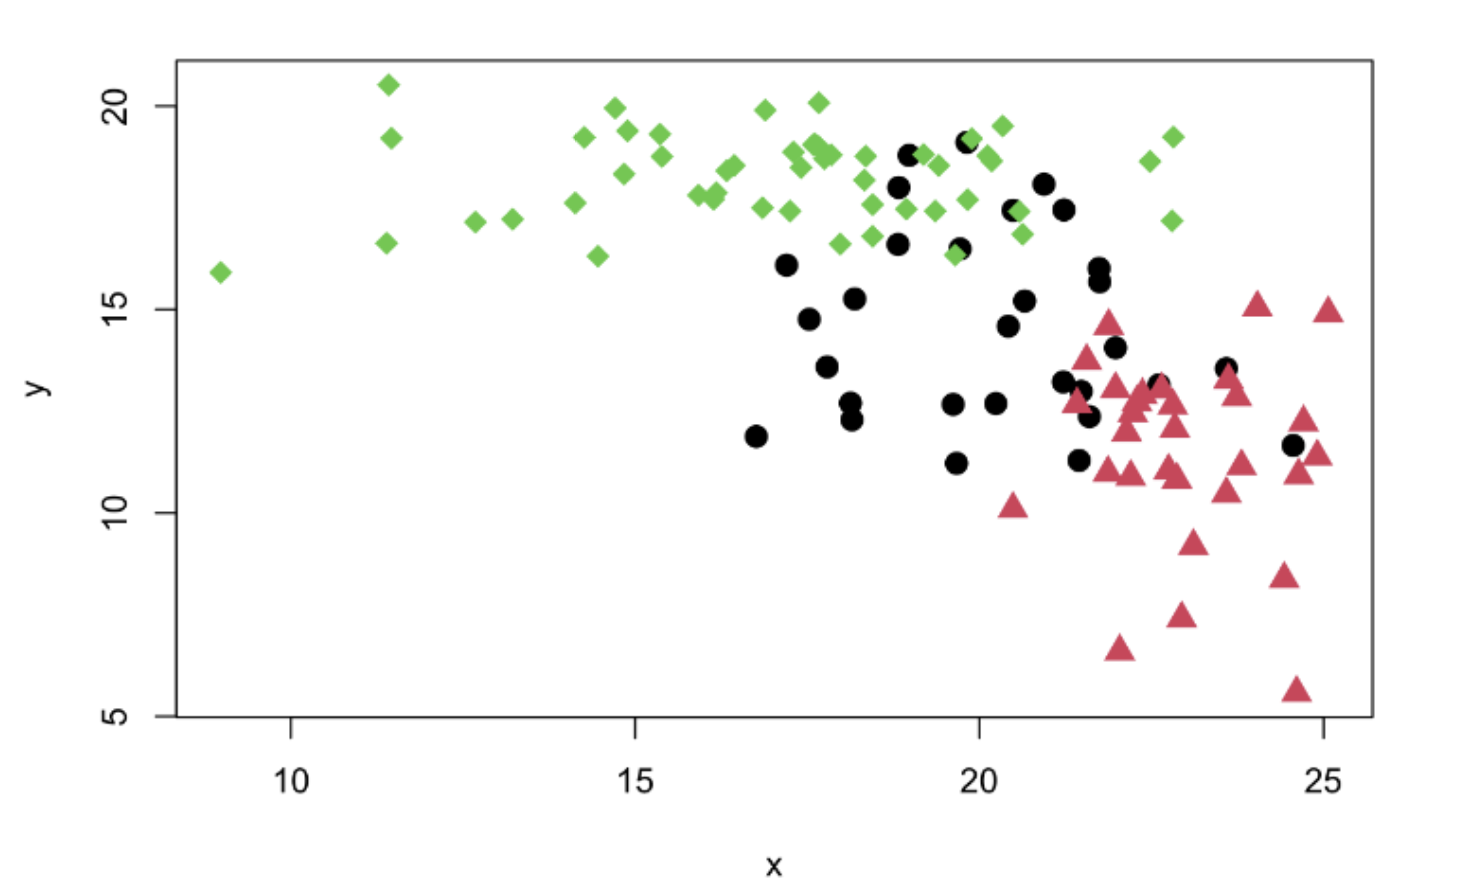
\includegraphics[width = \textwidth]{Rplot1.png}
    \end{center}
  \end{figure}
  Using a 60\%, 40\% split for our train and test data with proportional priors we achieved an accuracy 72.73\% with the multinomial logistic regression model.\\ 
  \textbf{Code:}
  \begin{center}
  \lstinputlisting[basicstyle = \footnotesize]{r5.txt}
  \end{center}

  
\end{exercise}
\vspace{1in}



\begin{exercise}{4}  Now for a nonparametric approach to discriminant analysis (other ones include Neural Nets and Kernel Discriminant
  Analysis). First, load the second data set from the APPENDIX.\\
  \begin{enumerate}
    \item[a.] First, plot w1 vs w2 using plot(w1,w2,pch=group). Do you see potential trouble in the discriminant analysis?\\
    \solution Plotting the data we find that the two groups somewhat overlap and are most definitely not linearly separable. 
    We can see that one of the groups is a lot closer together towards the center of the plot. A good discriminant 
    analysis will need to be flexible to identify the circular boundary between the two groups. 

    \begin{figure}[H]
      \begin{center}
        \caption{Data From Appendix}
      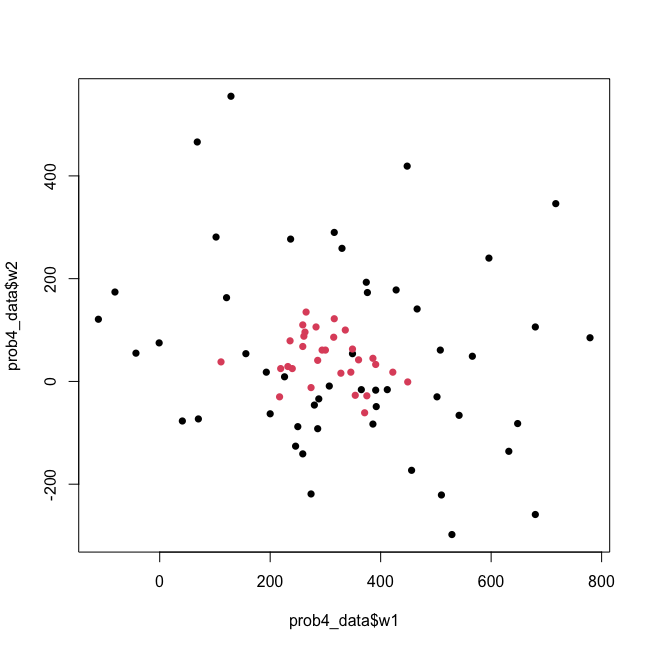
\includegraphics[width = .60\textwidth]{Rplot01.png}
      \end{center}
    \end{figure}
       \begin{footnotesize}
       \begin{verbatim}
        plot(prob4_data$w1,prob4_data$w2,col=prob4_data$group, pch = 16)
       \end{verbatim} 
       \end{footnotesize}

    \vspace{.15in}


    \item[b.] Now load the library 'rpart'. Run the following code that will produce a classification tree:\\
      \begin{footnotesize}
      \begin{verbatim}
        library(rpart)
        tree_output <- rpart(group~w1+w2,method="class",data=prob4_data)
        plot(tree_output)
        text(tree_output, use.n=TRUE)
        predict(tree_output)
        table(predict(tree_output)[,1]<0.5, prob4_data$group) # I swapped these around. Truth goes along the top. 
      \end{verbatim} 
      \end{footnotesize}
      The last step produces a classification table, where the first column of predict(hold) is actually the probability that the item belongs to group 2 (I
      warned you that these programs pick which is the first group and which is the second group, and don't always do it the way you want)! Did this
      do a good job of classification?\\
      \solution Running the code we produce the following figure and confusion matrix, 
      \begin{figure}[H]
        \begin{center}
          \caption{Decision Tree Classifier}
        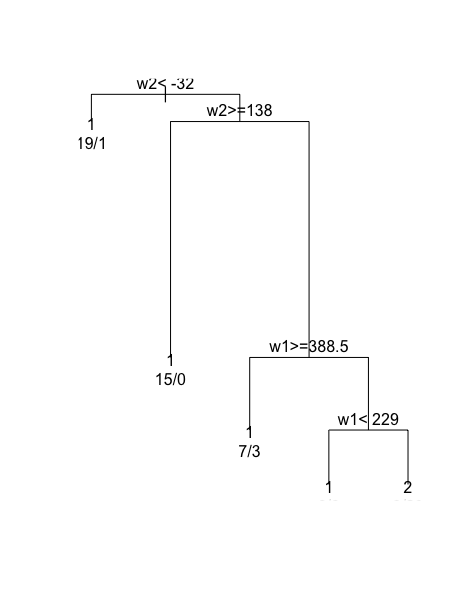
\includegraphics[width = \textwidth]{Rplot02.png}
        \end{center}
      \end{figure}
      \textbf{Code:}
      \begin{center}
      \lstinputlisting[basicstyle = \footnotesize]{r6.txt}
      \end{center}
      The decision tree model achieved an accuracy of 87.5\% on the data. Scanning through the rpart.control documentation we can see the default hyperparameters that where used to 
      build the tree. Looking at the tree alone, we can see that the decision boundary is simply a box around a majority of the interior group. Even though we have an accuracy of 87.5\% 
      this decision boundary suggests to me that the model is underfit. I think with more relaxed hyperparameters we could achieve a more circular rectilinear boundary which more closely 
      approximates the circular shape of the two groups. Boosting or Bagging the models would also achieve this effect. 
      \vspace{.15in}

      \item[c.]Look at the tree. On the original plot of w1 vs w2, try to find the region of the graph that will be assigned to group 2 (do this by reading the
      tree diagram).\\
      \solution Like we mentioned in the previous section, the decision boundary is simply a square. We can visualize it by using the tree and the abline() function. Doing so we get the following, 
      \begin{figure}[H]
        \begin{center}
          \caption{Decision Tree Classifier Boundary}
        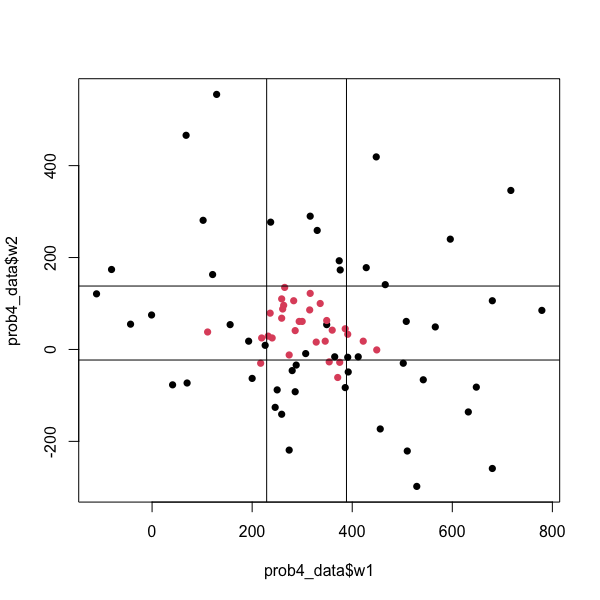
\includegraphics[width = \textwidth]{Rplot03.png}
        \end{center}
      \end{figure}
      \textbf{Code:}
      \begin{center}
      \lstinputlisting[basicstyle = \footnotesize]{r7.txt}
      \end{center}


      







  \end{enumerate}
  
\end{exercise}





\end{document}


















